\documentclass[conference]{IEEEtran}

\IEEEoverridecommandlockouts

\usepackage[utf8]{inputenc}
\usepackage[T1]{fontenc}

\usepackage{cite}

\ifCLASSINFOpdf
  \usepackage[pdftex]{graphicx}

\else

\fi

\usepackage[cmex10]{amsmath}

\usepackage{multirow}
\usepackage{array}
\usepackage[lofdepth,lotdepth]{subfig}
\usepackage{color}
\usepackage{tabto}

\usepackage{amssymb}
\usepackage{booktabs}
\usepackage{multirow}
\usepackage{rotating}
\usepackage{amsmath}
\usepackage{algorithm}
\usepackage{algpseudocode}
\usepackage{lineno,hyperref}
\usepackage{graphicx}
\usepackage{pdflscape}
\usepackage[none]{hyphenat}

\begin{document}

\IEEEpubid{\makebox[\columnwidth]{\hfill} \hspace{\columnsep}\makebox[\columnwidth]{}}

\title{Kırmızı Şarap Kalitesinin Makine Öğrenmesi Kullanılarak Tahmin Edilmesi
\\
\*

Predicting Red Wine Quality Using Machine Learning
}
\author{
	
\IEEEauthorblockN{Samed ZIRHLIOĞLU}
\IEEEauthorblockA{Bilgisayar Mühendisliği\\
	18110131037\\
	Kahramanmaraş Sütçü İmam Üniversitesi\\
	Kahramanmaraş, Türkiye\\
	zirhlioglusamed@gmail.com
	}
\and
\IEEEauthorblockN{Mehtap ÖKLÜ}
\IEEEauthorblockA{Bilgisayar Mühendisliği\\
	17110131052\\
	Kahramanmaraş Sütçü İmam Üniversitesi\\
	Kahramanmaraş, Türkiye\\
	mehtap\_oklu\_06@hotmail.com
	}
}
\maketitle
\thispagestyle{plain}
\pagestyle{plain}
\begin{ozet}
Şarap, çok eski tarihlerden beri tüketilen, batı toplumlarında mutfakla özdeşleşmiş olan alkollü bir içecektir. Farklı meyvelerle üretilebiliyor olsa da, şarap denince akla ilk gelen meyve üzümdür. Şarap, çok geniş bir skalaya sahiptir. Bu yüzden her şarabın kalite oranı farklıdır. Üzümle üretilen şarap türlerinden birisi de kırmızı şaraptır. Kırmızı şaraba ait bazı öznitelikler (alkol oranı, pH, klorür vb.) incelenerek şarabın kalitesi tahmin edilebilir. Bu özniteliklerin incelenmesi için de belirlenen yapay zekâ algoritmaları (KNN, SVC, Lojistik Regresyon, Naive Bayes, Karar Ağacı, Bagging ve Rastgele Orman Ağacı) kullanılmıştır. Kullanılan algoritmaların geneli sınıflandırma algoritmalarıdır. Bunun sebebi, şarabın kaliteli veya kalitesiz (0-1) olarak etiketlenmek istenmesidir.
\end{ozet}

\begin{IEEEanahtar}
Kırmızı Şarap, Kalite, KNN, SVC, Lojistik Regresyon, Naive Bayes, Karar Ağacı, Bagging ve Rastgele Orman Ağacı
\end{IEEEanahtar}


\begin{abstract}
Wine is an alcoholic beverage that has been consumed since ancient times and has been identified with cuisine in western societies. Although it can be produced with different fruits, the first fruit that comes to mind when talking about wine is grapes. Wine has a very wide scale. Therefore, the quality ratio of each wine is different. One of the types of wine produced with grapes is red wine. The quality of red wine can be estimated by examining some of the attributes (alcohol content, pH, chloride, etc.). Artificial intelligence algorithms (KNN, SVC, Logistic Regression, Naive Bayes, Decision Tree, Bagging and Random Forest Tree) were used to examine these features. The general algorithms used are classification algorithms. This is because wine is wanted to be labeled as good quality or poor quality (0-1).
\end{abstract}

\begin{IEEEkeywords}
Red Wine, Quality, KNN, SVC, Logistic Regression, Naive Bayes, Decision Tree, Bagging, and Random Forest Tree
\end{IEEEkeywords}
\pagebreak
\section{\textbf{GİRİŞ}}
\quad Şarap, diğer adıyla mey. Parçalanmış veya parçalanmamış üzümün fermente edilmesiyle\cite{1} üretilen, tescillenmiş veya tescillenmemiş, \%9-15 oranda alkole sahip\cite{2} bir içecektir. Tescillenmiş şaraplar, üretildiği coğrafi bölgenin bir işaretini taşır\cite{3}.

\quad Şarap, bilinmeyen tarihlerden beri üretilen ve tüketilen bir içecektir. Elimizde bulunan bilgilere göre şu an şarabın bilinen doğum yeri Gürcistan’dır, tarihi ise MÖ 6000’lere kadar dayanmaktadır\cite{2}. Şarap, birden fazla çeşide sahiptir. Bunlar; kırmızı, beyaz, rose, blush, likor şarabı vb. şeklindedir\cite{1}. Bu makalede kırmızı şarap incelenecektir.

\quad Şarap üretimi çok fazla emek isteyen, yorucu bir iştir. Gerek ilkel yöntemlerle, gerek de modern teknolojiyle şarap üretmek mümkündür. Şarap üretiminde yer alan bu teknolojinin ilerlemesiyle birlikte, şarap kalitesiyle alakalı kriterler de daha detaylı hale gelmiştir\cite{1}. Bu kriterler ve parametreler(uçucu asitlik, artık şeker miktarı, alkol oranı, pH, klorür vb.) daha net bir şekilde incelenebildiği için şarabın kalitesiyle ilgili ölçümler de daha rahat yapılabilmektedir. Bu makalede de yapay zeka kullanarak kırmızı şarap kalitesi ölçülmeye çalışılacaktır.

\quad Kırmızı şarap üzerinde kimyasal ölçümler yapılarak bir takım veriler elde edildi. Bu veriler Kaggle\cite{4}'da açık kaynak olarak paylaşılmıştır. Bu veri seti edinildi, üzerinde ön işleme yapıldı ve makine öğrenmesi algoritmaları kullanıldı. Bu makalede makine öğrenmesi kullanılarak kırmızı şarap kalitesi tahmin edilmeye çalışıldı.

\newpage

\quad Bu projede “Red Wine Quality” isimli veri seti\cite{4} Kaggle üzerinden temin edildi. Verinin \%30 test, \%70’i de eğitim için kullanıldı. Veri setinde 11 adet öznitelik, 1600 adet kayıt bulunmaktadır. Bu öznitelikler:

\begin{itemize}
  \item \textbf{fixed acidity (sabit asitlik): } Şarapla ilgili sabit, uçucu olmayan asitler. Kolayca buharlaşmazlar\cite{5}.
  \item \textbf{volatile acidity (uçucu asitlik): } Şarapta yüksek seviyelerde bulunduğunda sirke tadını ortaya çıkmasına neden olabilir\cite{5}.
  \item \textbf{citric acid (sitrik asit): } Şarapta az miktarda bulunduğunda daha taze ve fresh bir tat verir\cite{5}.
  \item \textbf{residual sugar (artık şeker): } Fermantasyon işleminden sonra arta kalan şeker miktarı, 1 g/L’den az olan şaraplar nadir bulunur. 45 g/L’den fazla şaraplar sweet(tatlı) olarak kabul edilir\cite{5}.
  \item \textbf{chlorides (klorür): } Şaraptaki tuz miktarıdır\cite{5}.
  \item \textbf{free sulfur dioxide (serbest kükürt dioksit): } Serbest form halinde bulunan kükürt dioksit, çözünmüş bir gaz ve bisülfit iyonu arasında dengede kalır.. Şarap oksidasyonunu önleme yanında büyümeyi (mikrobiyal) sağlar\cite{5}.
  \item \textbf{total sulfur dioxide (toplam kükürt dioksit): } Düşük seviyelerde, şarapta anlaşılması zordur fakat 50PPM’yi geçtiği zaman şarabın kokusunda ve tadında belirgin hale gelir\cite{5}.
  \item \textbf{density (yoğunluk): } Şarabın yoğunluğu 1.08 - 1.09 civarındadır. Bu durum da şarabın suya göre \%8-9 daha yoğun olduğu anlamına gelir\cite{6}.
  \item \textbf{pH (asidik-bazik): } pH cetvelinde 0-14 arasında değerde  şarabın asitlik ve baziklik değerini verir. Şaraplar pH cetvelinde 3-4 arasında yer alır\cite{5}.
  \item \textbf{sulphates (sülfür): } Antimikrobiyal ve antioksidan görevi gören kükürt dioksit gazının (SO2) seviyelerine katkıda bulunabilen bir katkı maddesidir\cite{5}.
  \item \textbf{alcohol: } Şarabın yüzde kaç alkol içerdiğini gösterir. Kırmızı şarapta alkol oranı \%11-14 arasındadır\cite{5}.
\end{itemize}

\quad Bu veri setinde kalite sütunu yani sonuç özniteliğinde 0-1 değerleri yer almaktadır. Öznitelikler doğrultusunda şarabın yüksek veya düşük kaliteli olduğu belirtilmektedir. Elimizde bulunan bu veri setinde en verimli şekilde etiketleme yapabilmek için; KNN, SVC, Lojistik Regresyon, Naive Bayes, Karar Ağacı, Bagging ve Rastgele Orman Ağacı algoritmaları kullanıldı. Proje; Python dilinde, Anaconda-Spyder editöründe yazıldı.
\pagebreak
\begin{figure}[!h]
	\centering%
	%\scriptsize
	\begin{center}
		\begin{tabular}{cc}%
			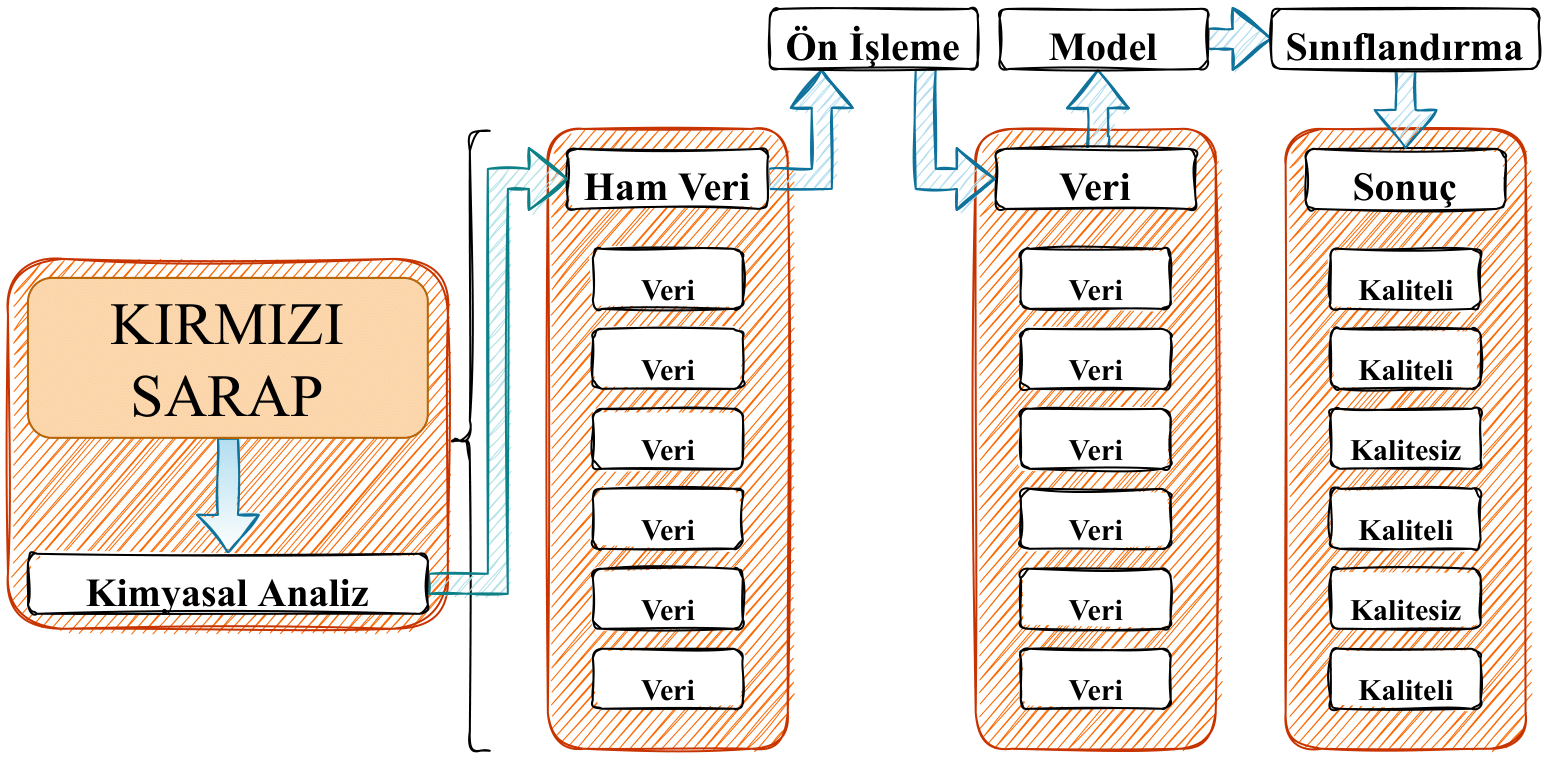
\includegraphics[scale=0.2]{pictures/pic_01.png}&%
		\end{tabular}%
	\end{center}
	\caption{Kırmızı Şarap Kalite Kontrol Süreci}%
	\label{fig:01}
\end{figure}

Projenin akış diyagramı Şekil \ref{fig:01}'deki gibidir. Makalenin ikinci bölümünde, bahsedilen algoritmalar hakkında bilgiler sunulmaktadır. Daha sonraki bölümde ise sonuçlar yer almaktadır.

\section{\textbf{METODLAR}}
\quad Kırmızı şarap kalitesini tahmin edebilmek için belirlenen sınıflandırma algoritmaları kullanıldı. Bu algoritmalar aşağıdaki gibidir.
\subsection{\textbf{K-Nearest Neighbor}}
\quad Gözetimli (denetimli) öğrenme metotlarından olup basit sınıflandırma işlemlerinde kullanılır\cite{8}\cite{9}.Sınıflandırma çalışması yaparken elimizdeki veriler hakkında kısıtlı ön bilgiye sahip olduğumuzda tercih etmemiz gereken ilk algoritmalardan biridir\cite{8}.

\begin{figure}[!h]
	\centering%
	%\scriptsize
	\begin{center}
		\begin{tabular}{cc}%
			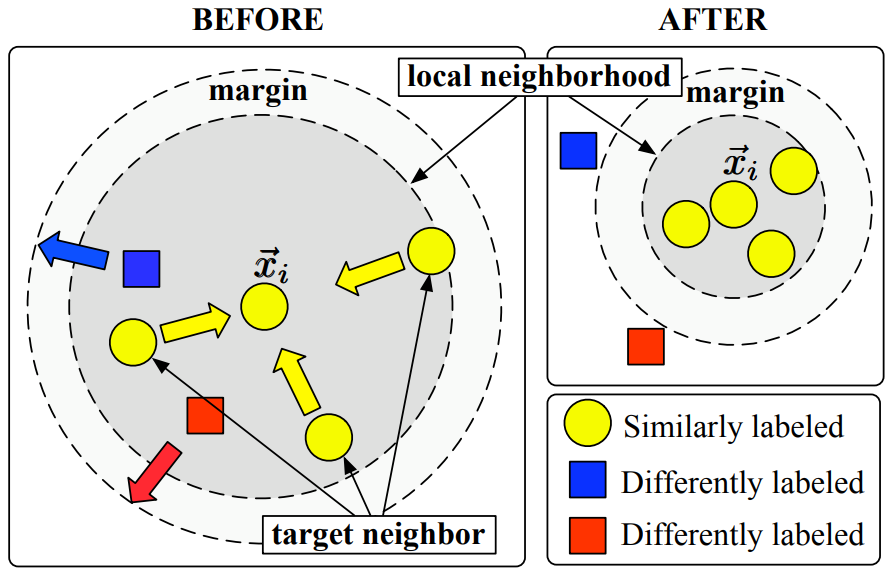
\includegraphics[scale=0.3]{pictures/pic_02.png}&%
		\end{tabular}%
	\end{center}
	\caption{Örnek KNN Şeması\cite{10}}%
	\label{fig:02}
\end{figure}

\quad Bu algoritmanın performansını etkileyen parametreler; uzaklık ölçütü, komşu sayısı(k) ve ağırlıklandırma yöntemidir\cite{7}. Uzaklık ölçütü olarak Manhattan uzaklığı kullanıldı(\textbf{n} boyutlu düzlemdeki iki konum arasındaki farkların, mutlak değerlerinin toplamı). X-Y konumları arasındaki Manhattan uzaklığı: P=(x1, x2,…, xn) ve Q=(y1, y2,…, yn) olmak üzere, Eşitlik \ref{eq:01}'e göre hesaplanır\cite{7}.

\begin{equation}
\label{eq:01}
\Large \sum_{i=1}^{n}\left | x_{i} - y_{i} \right |
\end{equation}

\pagebreak
KNN algoritmasının aşamaları\cite{9}:
\begin{itemize}
\item K değeri belirlenir
\item Diğer konumlara olan uzaklık, Manhattan yöntemiyle hesaplanır
\item Uzaklıklar sıralanarak en yakın komşular bulunur
\item En yakın K adet komşunun kategorileri toplanır
\item Toplam sonucunda ağırlıkta olan kategori seçilerek etiketleme yapılır
\end{itemize}

\subsection{\textbf{Support Vector Machines (SVM)}}
\quad Türkçe adıyla Destek Vektör Makineleri (DVM), istatistiksel öğrenme teorisi geliştiricisi Vapnik tarafından geliştirilmiştir. Sınıflandırma, örüntü tanıma problemleri için kullanılır. Destek Vektör Makineleri, alanındaki birçok tekniğe göre daha yüksek başarı oranına sahiptir. Uygulama sırasında çekirdek fonksiyon seçimi ve parametre optimizasyonu çok önemlidir\cite{11}.

\begin{figure}[!h]
	\centering%
	%\scriptsize
	\begin{center}
		\begin{tabular}{cc}%
			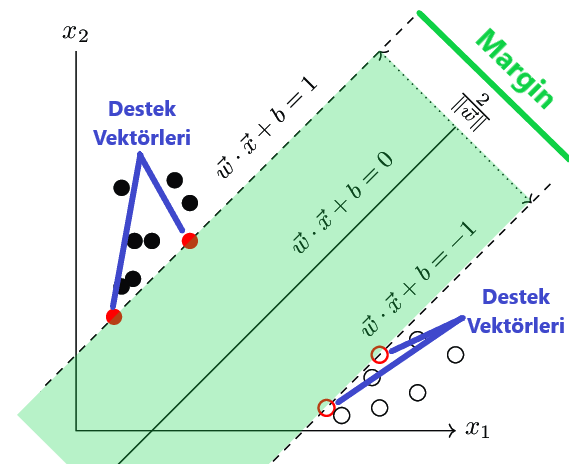
\includegraphics[scale=0.3]{pictures/pic_03.png}&%
		\end{tabular}%
	\end{center}
	\caption{Örnek SVM Şeması\cite{12}}%
	\label{fig:03}
\end{figure}

Şekil \ref{fig:03} üzerinde siyah ve beyaz olmak üzere iki sınıf mevcuttur. Gelecek verilerin sınıflandırılabilmesi için öncelikle sınıfları birbirinden ayıran bir doğru çizilir. Bu doğrunun -1 ve +1 değerleri arasında kalan yeşil kısım Margin bölgesidir. Margin ne kadar geniş olursa, sınıflar o kadar iyi ayrışıyor demektir. Bu işlemin formülü Eşitlik \ref{eq:02}'deki gibidir.

\begin{equation}
\label{eq:02}
\Large \hat{y}=\left\{\begin{matrix} 0, w^{T} \cdot x + b < 0,\\ 1, w^{T} \cdot x + b \geq 0 \end{matrix}\right.
\end{equation}

\quad Elde edilen sonuç 0’dan küçük çıkarsa beyaz noktaların bulunduğu kısma yakın olacaktır. Sonuç 0’a eşit veya 0’dan büyük çıkarsa siyah noktaların bulunduğu kısma daha yakın olacaktır\cite{12}.
\pagebreak
\subsection{\textbf{Logistic Regression}}

\quad Lojistik Regresyon, sonucu 0 veya 1 şeklinde üreten, değişkenlerin modellenmesinde kullanılan algoritmadır. Örneğin kırmızı şarap kalitesi ele alındığında; eldeki veri setinde 0 kalitesiz, 1 kaliteli durumunu temsil eder. Yani Lojistik Regresyon algoritmasıyla verilerin ait oldukları sınıflar tahmin(predict) edilebilir\cite{13}.

\begin{equation}
\label{eq:03}
\Large f(x)=\frac{1}{1+e^{-z}}
\end{equation}

Lojistik regresyon, $\left(-\infty,+\infty \right)$ aralığındaki değerleri girdi olarak kabul eder\cite{13}.

\begin{figure}[!h]
	\centering%
	%\scriptsize
	\begin{center}
		\begin{tabular}{cc}%
			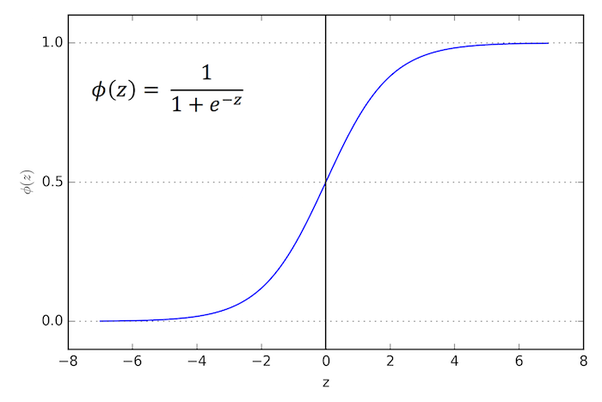
\includegraphics[scale=0.3]{pictures/pic_04.png}&%
		\end{tabular}%
	\end{center}
	\caption{Örnek bir Lojistik Regresyon Şeması\cite{13}}%
	\label{fig:04}
\end{figure}

\subsection{\textbf{Naive Bayes}}
\quad Naive Bayes algoritması sınıflandırıcı teorem olan Bayes’e dayanmaktadır\cite{15}. Adını İngiliz matematikçi olan Thomas Bayes’ten almıştır\cite{14}. Naive Bayes, elimizdeki örneklerin hangi sınıfa ait olduğunu, işlemler sonucu elde ettiği oranla tahmin eder. Naive Bayes’ın iki önemli kabulü vardır\cite{15}. Bunlar:
\begin{itemize}
\item Elimizde bulunan niteliklerin hepsi aynı derecede önemlidir.
\item Elimizde bulunan nitelikler birbirinden bağımsızdır.
\end{itemize}

\quad Koşullu olasılıklar arasında bağlantı kuran Bayes Teoremi, x özniteliğinin gerçekleşmiş olması durumunda C özniteliğinin gerçekleşmesi veya C özniteliğinin gerçekleşmiş olması durumunda x özniteliğinin gerçekleşmesi durumunu verir\cite{15}. Bayes kuralının algoritması Eşitlik \ref{eq:04}'deki gibidir. Eşitlikte yer alan değerler\cite{14}:

\begin{itemize}
\item \textbf{p(x|Cj):} j sınıfından bir örneğin x olma olasılığı
\item \textbf{P(Cj):} j sınıfının ilk olasılığı
\item \textbf{p(x):} Herhangi bir örneğin x olma olasılığı
\item \textbf{P(Cj|x):} x olan bir örneğin j sınıfından olma olasılığı (son olasılık)
\end{itemize}

\begin{equation}
\label{eq:04}
\Large P(C_{j}|x) = \frac {p(x|C_{j}) P(C_{j})} {p(x)} = \frac {p(x|C_{j}) P(C_{j})} {\sum_{k}^{}p(x|C_{k})P(C_{k})}
\end{equation}

\subsection{\textbf{Decision Tree}}
\quad Karar Ağacı, en yaygın kullanılan gözetimli(denetimli) öğrenme algoritmalarından birisidir. Adından da anlaşılacağı üzere ağaç tabanlı öğrenmeye dayalıdır. Tüm problemlere uyarlanabilir\cite{16}. Karar ağacı, kök düğüm değişkeninden başlayarak, ağaç dalı hiyerarşisi gibi dallanır\cite{17}.

\begin{figure}[!h]
	\centering%
	%\scriptsize
	\begin{center}
		\begin{tabular}{cc}%
			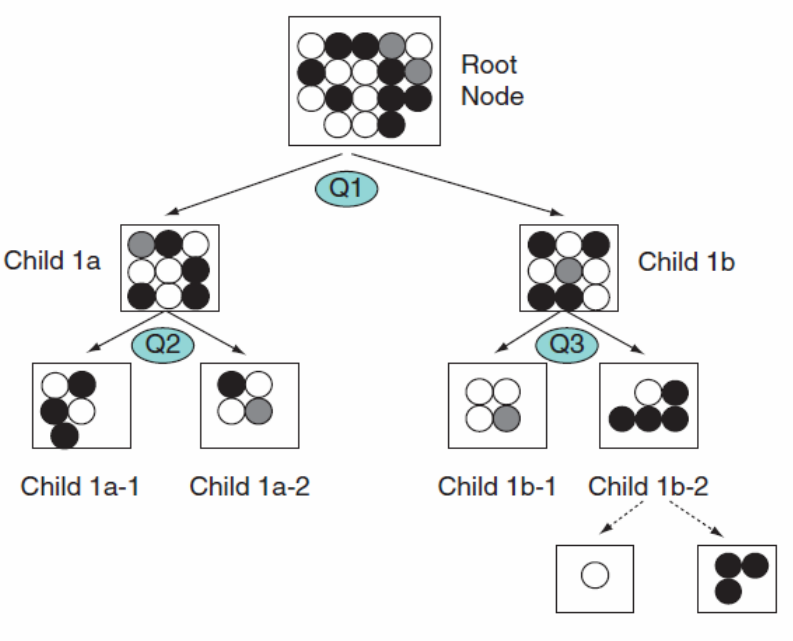
\includegraphics[scale=0.4]{pictures/pic_05.png}&%
		\end{tabular}%
	\end{center}
	\caption{Örnek bir Karar Ağacı Şeması\cite{17}}%
	\label{fig:05}
\end{figure}

\quad Entropi, verilerin belirsizliğinin bir ölçüsüdür; dolayısıyla entropinin düşük olması tercih edilir. Verilerin tamamı sezgisel olarak aynı etikete sahipse, veri setinin entropisi düşüktür denilebilir\cite{16}.

\begin{equation}
\label{eq:05}
\Large H=-\sum p(x)\log{p(x)}
\end{equation}

\quad Burada; p(x) belirli bir sınıfa ait grubun yüzde oranını, H ise entropiyi belirtmektedir. Karar Ağacı, entropiyi en aza indirecek şekilde bölünme yapmalıdır. En iyi bölümlemeyi belirlemek için kullanılan bilgi kazancı, Eşitlik \ref{eq:06}'daki gibi hesaplanır\cite{16}.

\begin{equation}
\label{eq:06}
\Large Gain(S,D) = H(S)-\sum_{V\in D}^{}\frac{\left|V\right|}{\left|S\right|}H(V)
\end{equation}

\quad Burada; \textbf{S} orijinal veri kümesini, \textbf{D} ise kümenin bölünmüş bir parçasını temsil eder. Her \textbf{V} değeri, \textbf{S}'nin alt kümesidir\cite{16}.
\pagebreak
\subsection{\textbf{Bagging (Torbalama)}}
\quad 1996 yılında Breiman tarafından geliştirilmiştir. Bagging algoritmasının çalışma biçimi Şekil \ref{fig:06}'da belirtilmiştir. Şekil \ref{fig:06}'daki aşamaların açıklamaları\cite{18}:

\begin{itemize}
\item \textbf{Bootstrap sampling:} Orijinal veri kümesi, alt kümelere bölünür.
\item \textbf{Model training:} Bu alt kümelerin her birinde ayrı ayrı temel (zayıf) model oluşturulur.
\item \textbf{Model forecasting:} Modeller birbirinden bağımsız ancak paralel olarak çalışır.
\item \textbf{Result aggregating:} Tüm modellerin tahmin sonuçları birleştirilerek niai tahmin belirlenir.
\end{itemize}

\begin{figure}[!h]
	\centering%
	%\scriptsize
	\begin{center}
		\begin{tabular}{cc}%
			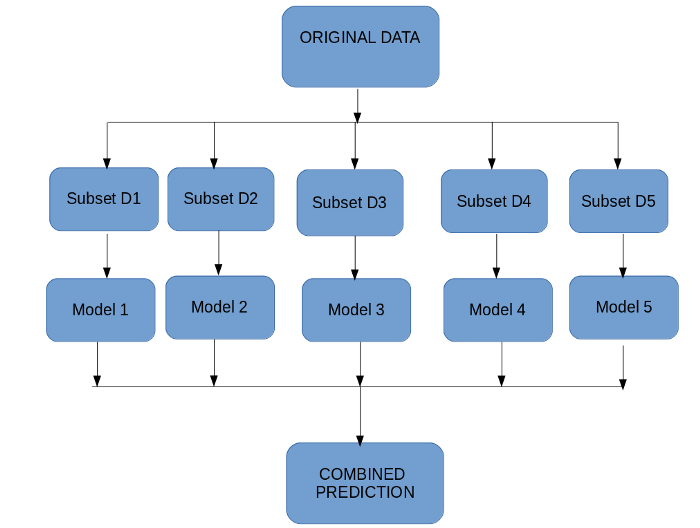
\includegraphics[scale=0.35]{pictures/pic_06.png}&%
		\end{tabular}%
	\end{center}
	\caption{Örnek bir Torbalama Şeması\cite{18}}%
	\label{fig:06}
\end{figure}
\newpage
\subsection{\textbf{Random Forest Tree (Rastgele Orman Ağacı)}}
\quad Denetimli bir sınıflandırma algoritmasıdır. Adından da anlaşılacağı gibi, algoritma rastgele bir orman yaratır. Ormanda bulunan ağaç sayısı ile elde edilen çıktılar arasında doğrusal bir ilişki vardır. Ağaç sayısı arttıkça elde edilecek olan sonucun kesinliği de artar. Rastgele Orman Ağacı’nın, Karar Ağacı’ndan farkı; kök bulma ve düğümleri bölme işlemlerinin çalışıyor olmasıdır\cite{19}. Rastgele Orman Ağacı’nın şeması Şekil \ref{fig:07}'de verilmiştir.

\begin{figure}[!h]
	\centering%
	%\scriptsize
	\begin{center}
		\begin{tabular}{cc}%
			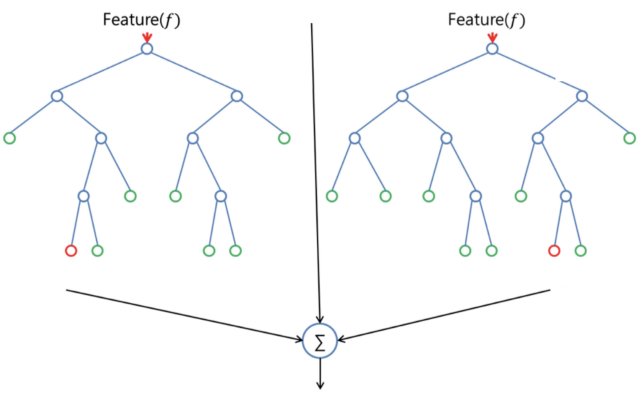
\includegraphics[scale=0.45]{pictures/pic_07.png}&%
		\end{tabular}%
	\end{center}
	\caption{Örnek bir Rastgele Orman Ağacı Şeması\cite{20}}%
	\label{fig:07}
\end{figure}

\quad Rastgele Orman Ağacı, kullanıcıdan iki parametre alır: m parametresi en iyi bölünmeyi belirlemek için her düğümde kullanılan değişkenlerin sayısı, N geliştirilecek ağaç sayısı. Öncelikle eğitim verilerinin 2/3'ü kullanılarak önyükleme örnekleri oluşturulur. Hata testi yapma amacıyla da geriye kalan 1/3'lük parça kullanılır. Bu parçaya ise \textbf{OOB (out of bag)} denir\cite{21}.

\quad Düğümlerdeki \textbf{m} değerleri, bütün değerlerin içinden rastgele bir şekilde seçilir. Böylece en iyi dal belirlenmiş olur. \textbf{M} adet değişkenin kareköküne eşit olarak alınan \textbf{m} değişkeni, genellikle optimuma en yakın sonucu verir\cite{21}.

\quad Sınıfların homojenliği $Gini$ indexi hesaplanarak ölçülür. $Gini$ indexi ne kadar düşükse, sınıf da o kadar homojendir. Bir düğümün alt $Gini$ indexi üst $Gini$ indexinden daha az olduğu durumlarda incelenen dal başarılı sayılır\cite{21}. $Gini$ indexinin formülü Eşitlik \ref{eq:07}'de verilmiştir. Formül değişkenlerinin temsil ettiği veriler de aşağıdaki gibidir;

\begin{itemize}
\item \textbf{T:} Tüm veri seti
\item \textbf{pj:} Veri kümesinde bulunan her verinin, kendinden küçük ve büyük eleman sayılarına bölümü
\item \textbf{n:} Seçilen verimiz
\end{itemize}

\begin{equation}
\label{eq:07}
\Large Gini(T)=1-\sum_{j=1}^{n}(p_{j})^{2}
\end{equation}

\pagebreak
\section{\textbf{SONUÇLAR}}

\quad Veri seti; $\%70$'i eğitim, $\%30$'u ise test için kullanılmak üzere iki parçaya ayrıldı. Oluşturulan model eğitim verisiyle eğitildi. Daha sonra test verisi ile predict(tahmin) işlemine tâbi tutuldu. Bu işlemler sonucunda elde edilen doğruluk$(acc)$ ve hata$(MSE)$ oranları Şekil \ref{fig:08}'deki grafiğe döküldü.

\begin{figure}[!h]
	\centering
	\begin{center}
		\begin{tabular}{cc}
			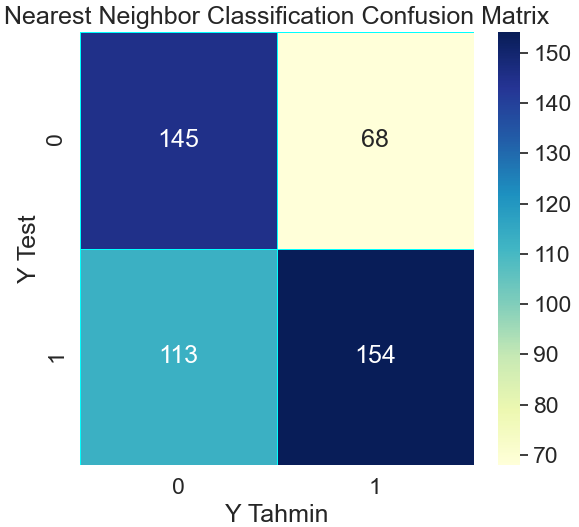
\includegraphics[scale=0.325]{pictures/pic_08.png}&
		\end{tabular}
	\end{center}
	\caption{Tüm Algoritmaların Doğruluk \& MSE Oranları}
	\label{fig:08}
\end{figure}

\quad Kırmızı şarap kalitesinin tahmin edilebilmesi için, "Red Wine Quality"\cite{4} isimli veri seti; Bagg, DT, KNN, LG, NB, RF ve SVM sınıflandırıcıları kullanılmıştır. Bu algoritmaların $acc$, $MSE$ ve $AUC$ değerleri, Tablo \ref{tbl:01}'de verilmiştir.

\begin{table}[h]
	\centering
	\small
	\begin{tabular}{|l|c|c|c|c|}
		\hline
					& \textbf{acc}	& \textbf{MSE}	& \textbf{AUC}	\\ \hline
		\textbf{Bagg}	& 0.7833		& 0.2166		& 0.785		\\ \hline
		\textbf{DT}		& 0.7645		& 0.2354 		& 0.760		\\ \hline
		\textbf{KNN}	& 0.7062		& 0.2937 		& 0.706		\\ \hline
		\textbf{LG}		& 0.7354		& 0.2645		& 0.736		\\ \hline
		\textbf{NB}		& 0.7416		& 0.2583		& 0.736		\\ \hline
		\textbf{RF}		& \textbf{0.8000}	& \textbf{0.2000}	& \textbf{0.796}	\\ \hline
		\textbf{SVM}	& 0.7583		& 0.2416		& 0.758		\\ \hline
	\end{tabular}
	\caption{Bagging, DT, KNN, LG, NB, RF ve SVM sınıflandırıcılarının \textit{acc, MSE ve AUC} ölçütlerinin ortalama değerleri}
	\label{tbl:01}
\end{table}

\quad Tablo \ref{tbl:01} incelendiği zaman, en yüksek doğruluk değerine $(acc)$ sahip olan algoritmanın Random Forest $(0.80)$ olduğu görülebilir. Bunu takip eden algoritma ise $0.7833$ doğruluk oranı ile Bagging Classifier’dır. Üçüncü sırada ise $0.7645$ doğruluk oranıyla Decision Tree yer almaktadır. Geriye kalan algoritmaların $acc$ değerlerine ise Tablo \ref{tbl:01}'de yer verilmiştir.

\quad $MSE$ (mean squared error/ortalama kare hatası) değerleri için; Tablo \ref{tbl:01} incelendiği zaman, en düşük $MSE$ değerine sahip olan algoritmanın Random Forest $(0.20)$ olduğu görülebilir. En yüksek $MSE$ değeri ise $0.2937$ oranıyla K-Nearest Neighbor algoritmasına aittir.

\pagebreak

\subsection{\textbf{Tüm Algoritmalara Ait ROC Eğrisi Grafiği}}

\quad Makine öğrenmesi algoritmalarının performans ölçümünde ROC eğrisinden de yararlanılır. Bu eğrilerin $AUC$(doğruluk) değerleri de mevcuttur ancak algoritmanın tahmin doğruluk skoruyla $(acc)$ karıştırılmamalıdır\cite{22}. Eldeki algoritmaların ROC eğrileri Şekil \ref{fig:09}'da verildi. Eğrilerin doğruluk oranları da Tablo \ref{tbl:01}'de belirtildi.

\begin{figure}[!h]
	\centering
	\begin{center}
		\begin{tabular}{cc}
			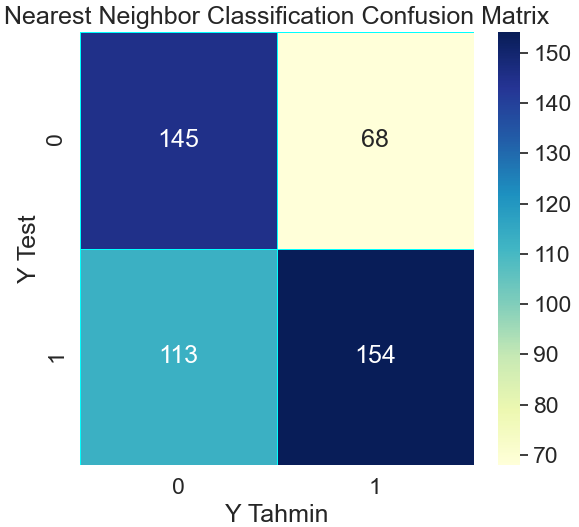
\includegraphics[scale=0.42]{pictures/pic_09.png}&
		\end{tabular}
	\end{center}
	\caption{Tüm Algoritmaların ROC Eğrileri ve AUC Değerleri}
	\label{fig:09}
\end{figure}

\subsection{\textbf{Confusion Matrix (Hata Matrisi)}}

\quad Tablo \ref{tbl:01}'de en yüksek doğruluk $(acc)$ değerine $(0.80)$ sahip olan Random Forest algoritması, yine aynı şekilde en düşük $(0.20)$ hata oranına $(MSE)$ da sahiptir. Doğruluk $(acc)$ ve hata $(MSE)$ değerleri arasında ters orantı vardır. Yani $acc$ değeri ne kadar yüksek olursa $MSE$ değeri de o kadar düşük olmaktadır.

\begin{itemize}
\item $acc + MSE = 1$
\end{itemize}

\begin{figure}[!h]
	\centering
	\begin{center}
		\begin{tabular}{cc}
			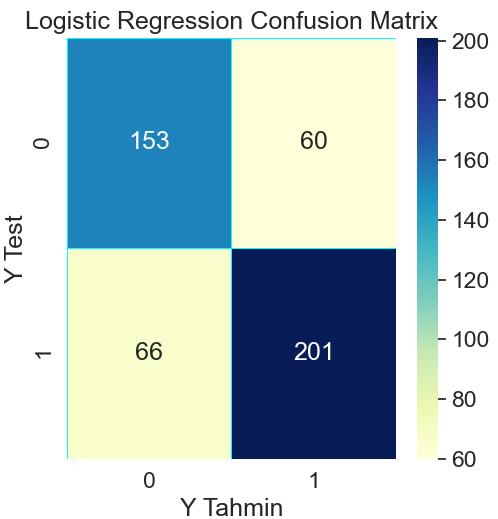
\includegraphics[scale=0.45]{pictures/pic_10.png}&
		\end{tabular}
	\end{center}
	\caption{K-Nearest Neighbor Hata Matrisi}
	\label{fig:10}
\end{figure}
\pagebreak
\begin{figure}[!h]
	\centering
	\begin{center}
		\begin{tabular}{cc}
			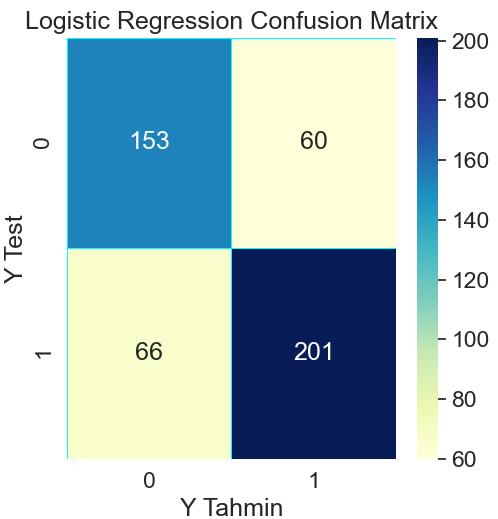
\includegraphics[scale=0.45]{pictures/pic_11.png}&
		\end{tabular}
	\end{center}
	\caption{Support Vector Machines Hata Matrisi}
	\label{fig:11}
\end{figure}

\begin{figure}[!h]
	\centering
	\begin{center}
		\begin{tabular}{cc}
			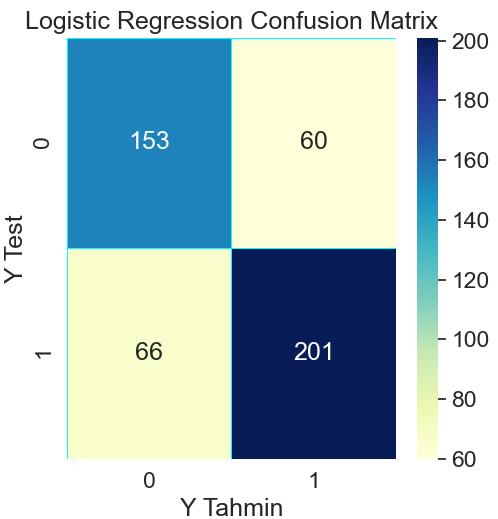
\includegraphics[scale=0.45]{pictures/pic_12.png}&
		\end{tabular}
	\end{center}
	\caption{Logistic Regression Hata Matrisi}
	\label{fig:12}
\end{figure}

\begin{figure}[!h]
	\centering
	\begin{center}
		\begin{tabular}{cc}
			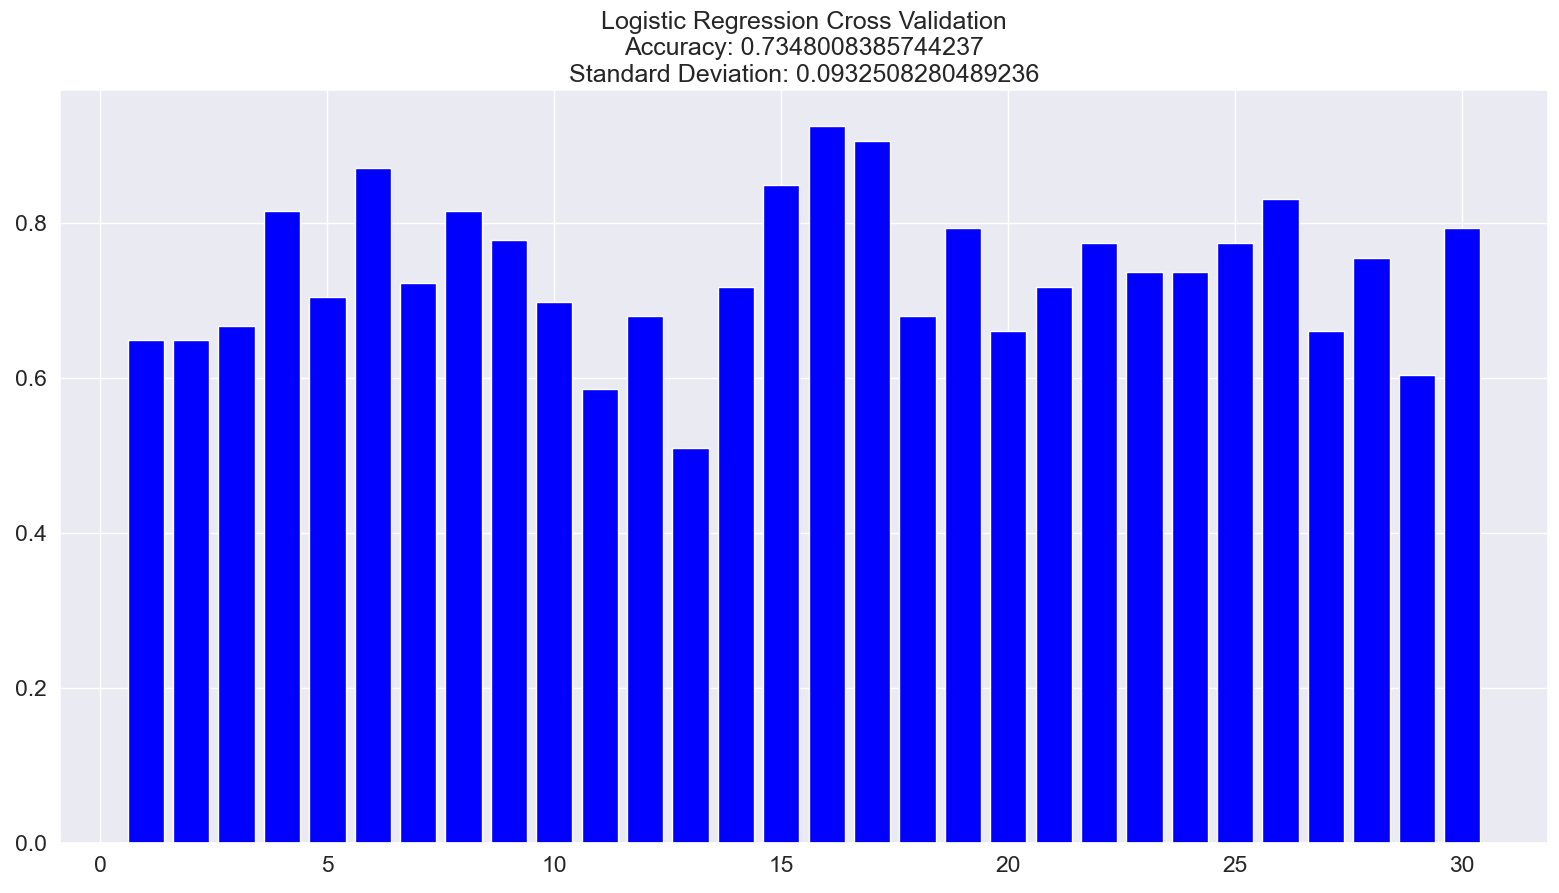
\includegraphics[scale=0.45]{pictures/pic_13.png}&
		\end{tabular}
	\end{center}
	\caption{Naive Bayes Hata Matrisi}
	\label{fig:13}
\end{figure}

\begin{figure}[!h]
	\centering
	\begin{center}
		\begin{tabular}{cc}
			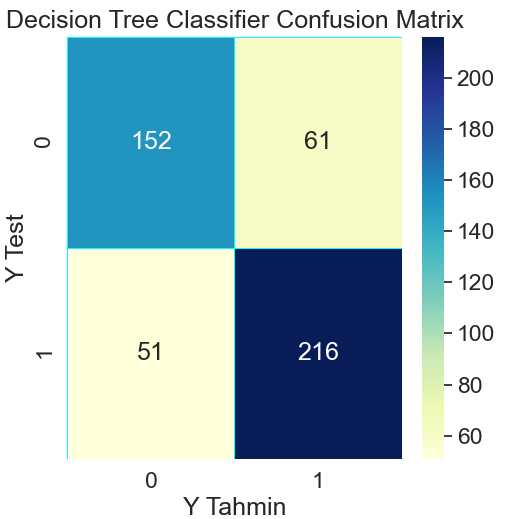
\includegraphics[scale=0.45]{pictures/pic_14.png}&
		\end{tabular}
	\end{center}
	\caption{Decision Tree Hata Matrisi}
	\label{fig:14}
\end{figure}

\begin{figure}[!h]
	\centering
	\begin{center}
		\begin{tabular}{cc}
			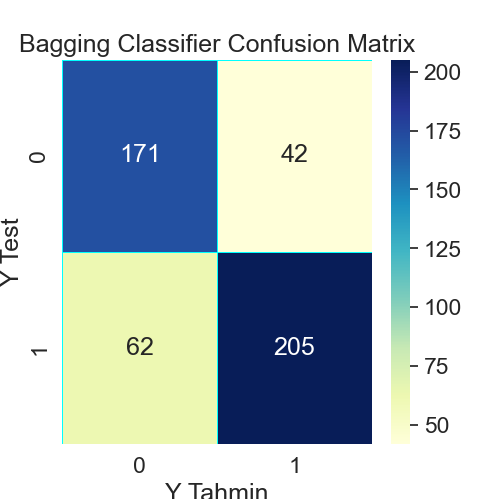
\includegraphics[scale=0.45]{pictures/pic_15.png}&
		\end{tabular}
	\end{center}
	\caption{Bagging Hata Matrisi}
	\label{fig:15}
\end{figure}
\pagebreak
\begin{figure}[!h]
	\centering
	\begin{center}
		\begin{tabular}{cc}
			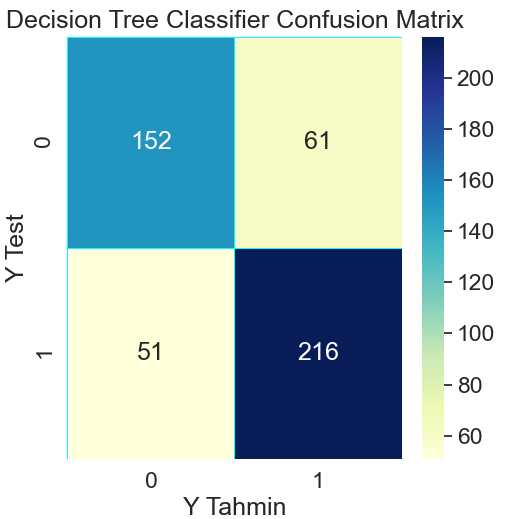
\includegraphics[scale=0.45]{pictures/pic_16.png}&
		\end{tabular}
	\end{center}
	\caption{Random Forest Tree Hata Matrisi}
	\label{fig:16}
\end{figure}
\pagebreak

\newpage
\subsection{\textbf{Cross-Validation (Çapraz Doğrulama)}}
\quad Cross-Validation, oluşturulan modelin birden fazla iterasyonda eğitilmesini sağlayan bir fonksiyondur. Normal çalıştırmalardan farkı, veri setindeki $train-test$ bölme işlemini her seferinde yeniden ve farklı bir şekilde yapıyor olmasıdır.

\quad Sınıflandırma algoritmaları bir kez eğitildi ve elde edilen veriler Tablo \ref{tbl:01}'de verildi. Bagg, DT, KNN, LG, NB, RF ve SVM algoritmalarının üzerinde, \textbf{10 Kat Çapraz Doğrulama} yöntemi kullanılarak 30 farklı koşma işlemi gerçekleştirildi. Bu koşma işlemlerinin tamamı rastgele ve birbirinden bağımsız olduğu için, farklı durumlarda algoritmaların nasıl çalıştığı da daha iyi anlaşılmış oldu.


\begin{figure}[!h]
	\centering
	\begin{center}
		\begin{tabular}{cc}
			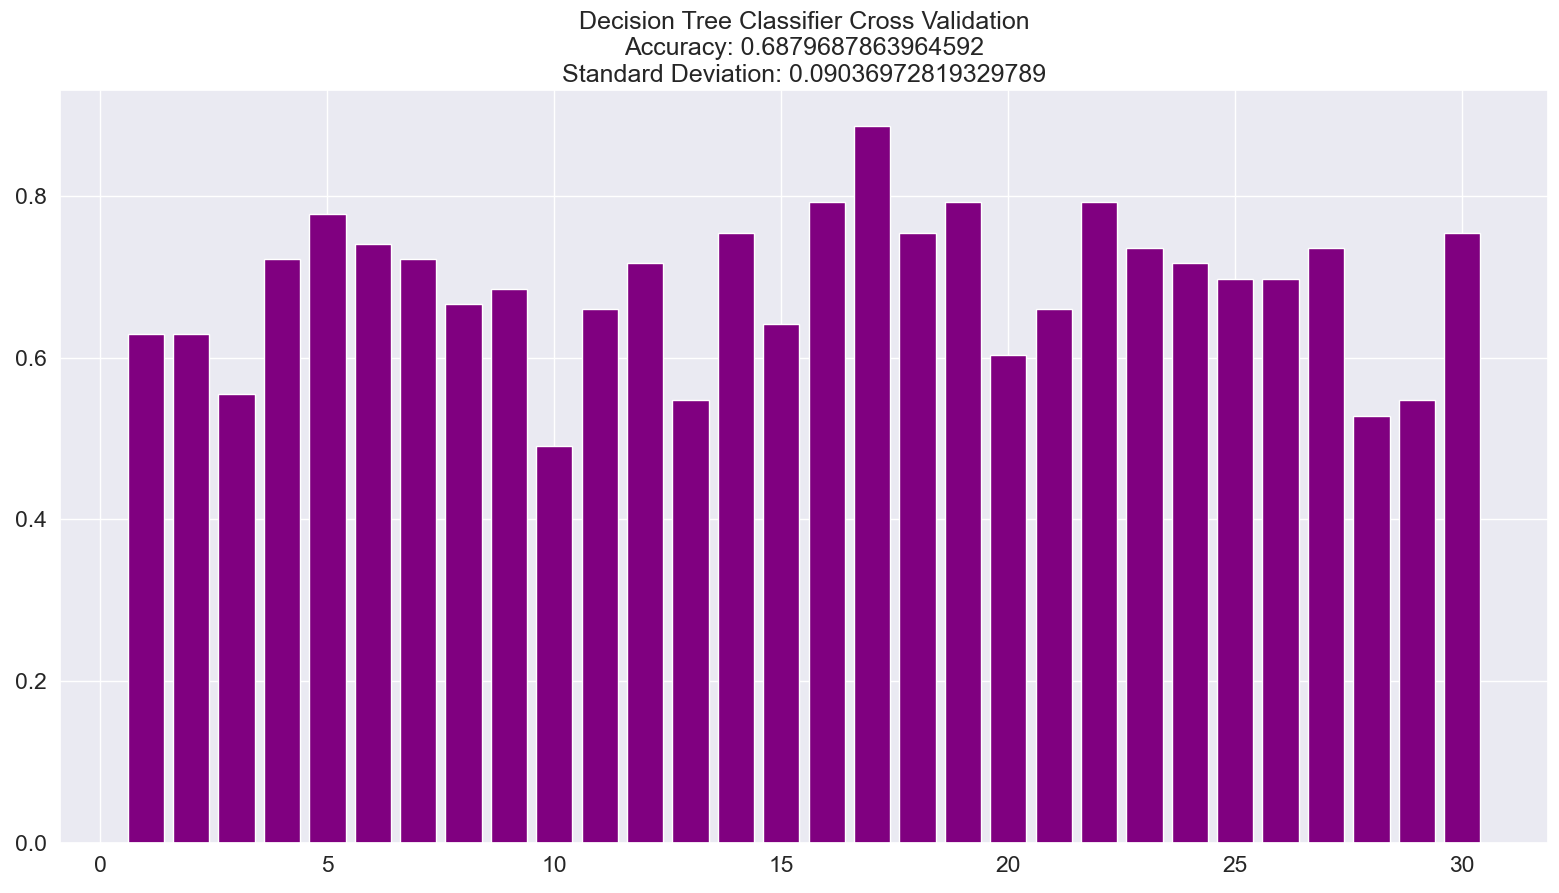
\includegraphics[scale=0.2]{pictures/pic_17.png}&
		\end{tabular}
	\end{center}
	\caption{K-Nearest Neighbor Cross-Validation}
	\label{fig:17}
\end{figure}

\begin{figure}[!h]
	\centering
	\begin{center}
		\begin{tabular}{cc}
			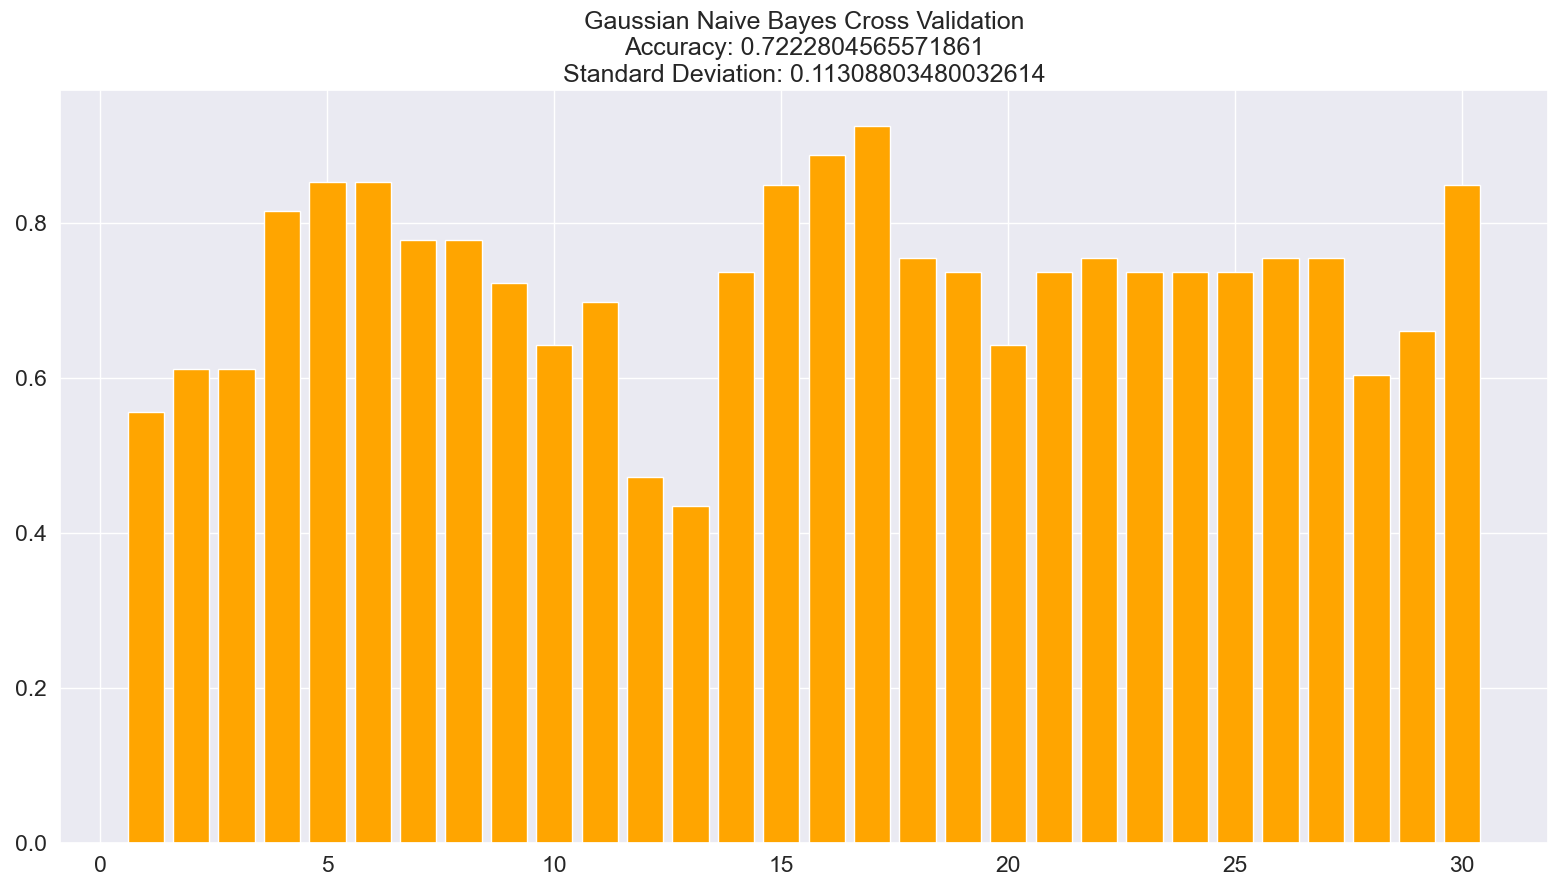
\includegraphics[scale=0.2]{pictures/pic_18.png}&
		\end{tabular}
	\end{center}
	\caption{Support Vector Machines Cross-Validation}
	\label{fig:18}
\end{figure}

\begin{figure}[!h]
	\centering
	\begin{center}
		\begin{tabular}{cc}
			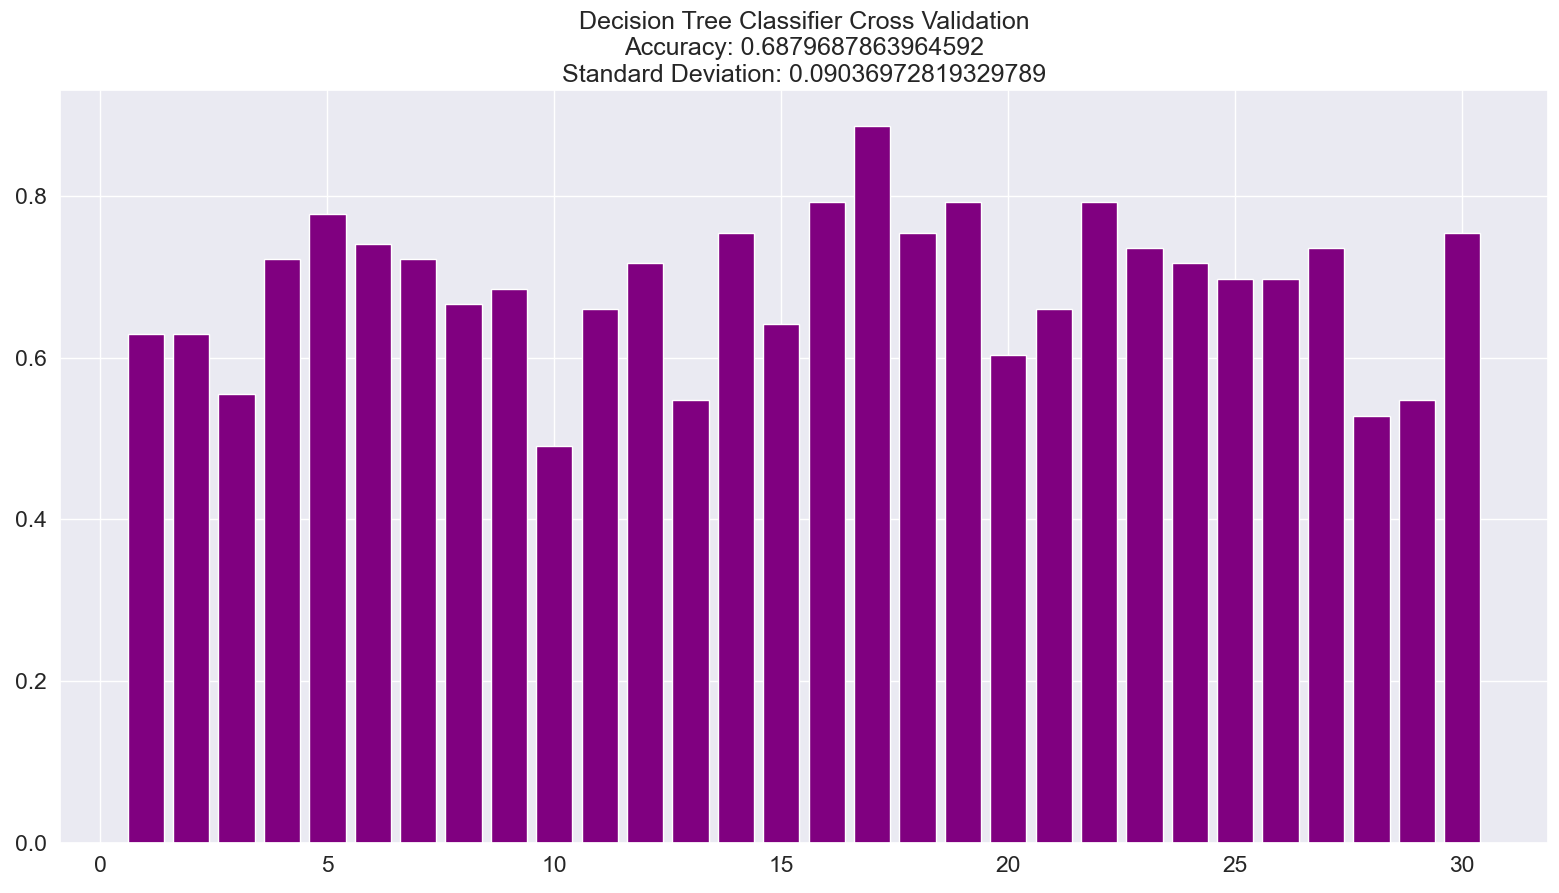
\includegraphics[scale=0.2]{pictures/pic_19.png}&
		\end{tabular}
	\end{center}
	\caption{Logistic Regression Cross-Validation}
	\label{fig:19}
\end{figure}
\pagebreak
\begin{figure}[!h]
	\centering
	\begin{center}
		\begin{tabular}{cc}
			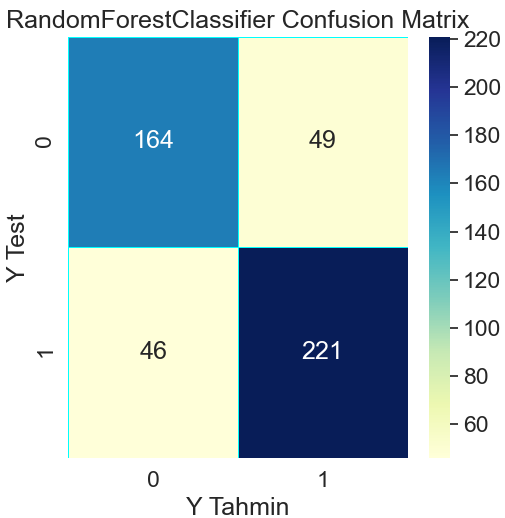
\includegraphics[scale=0.225]{pictures/pic_20.png}&
		\end{tabular}
	\end{center}
	\caption{Naive Bayes Cross-Validation}
	\label{fig:20}
\end{figure}

\begin{figure}[!h]
	\centering
	\begin{center}
		\begin{tabular}{cc}
			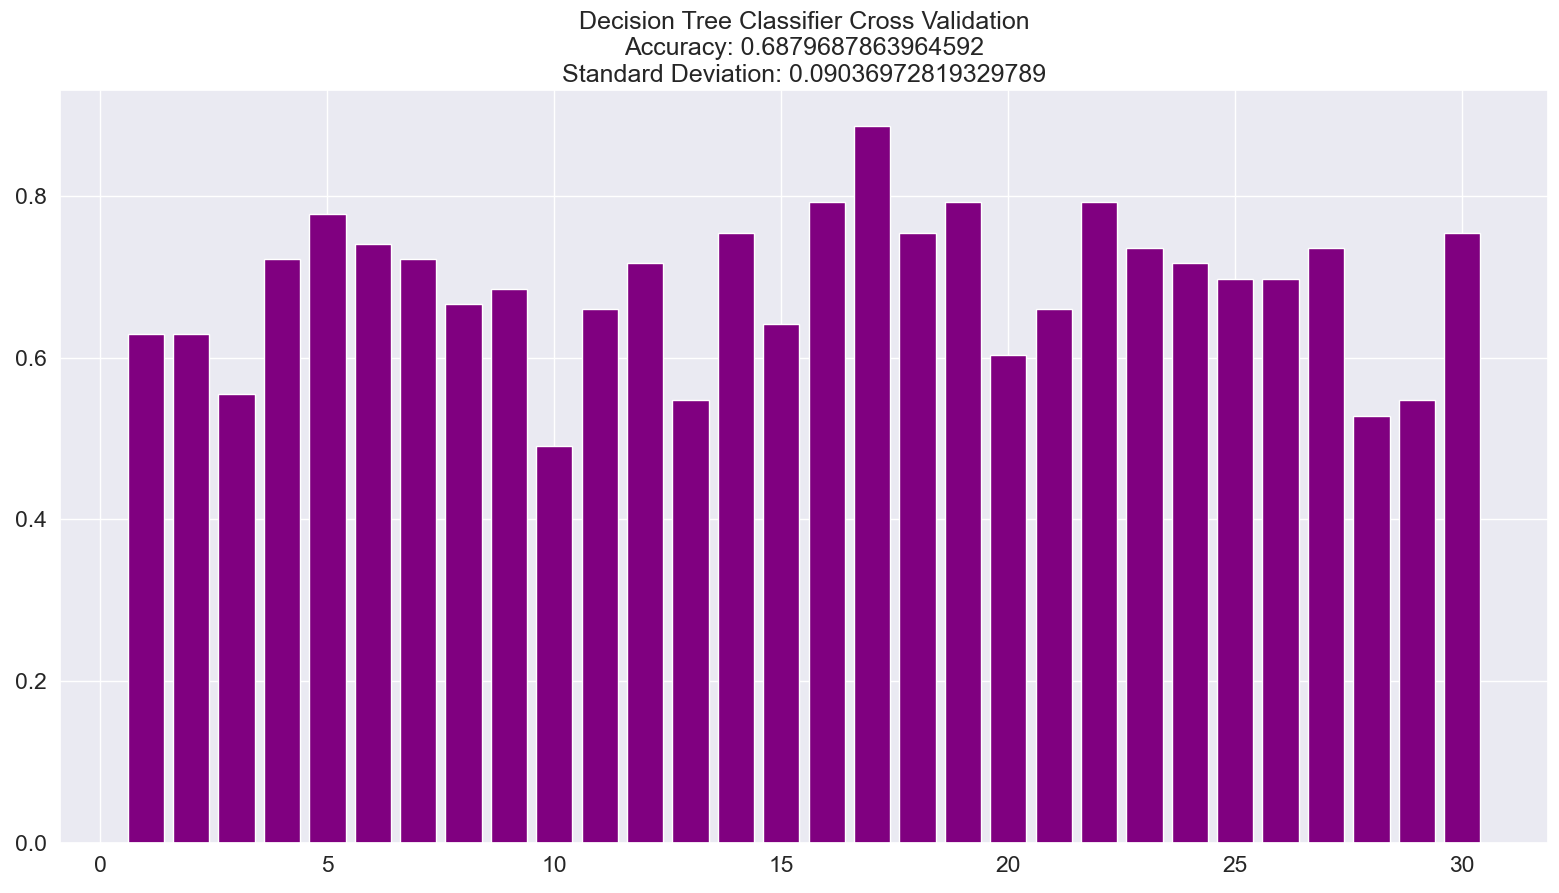
\includegraphics[scale=0.225]{pictures/pic_21.png}&
		\end{tabular}
	\end{center}
	\caption{Decision Tree Cross-Validation}
	\label{fig:21}
\end{figure}

\begin{figure}[!h]
	\centering
	\begin{center}
		\begin{tabular}{cc}
			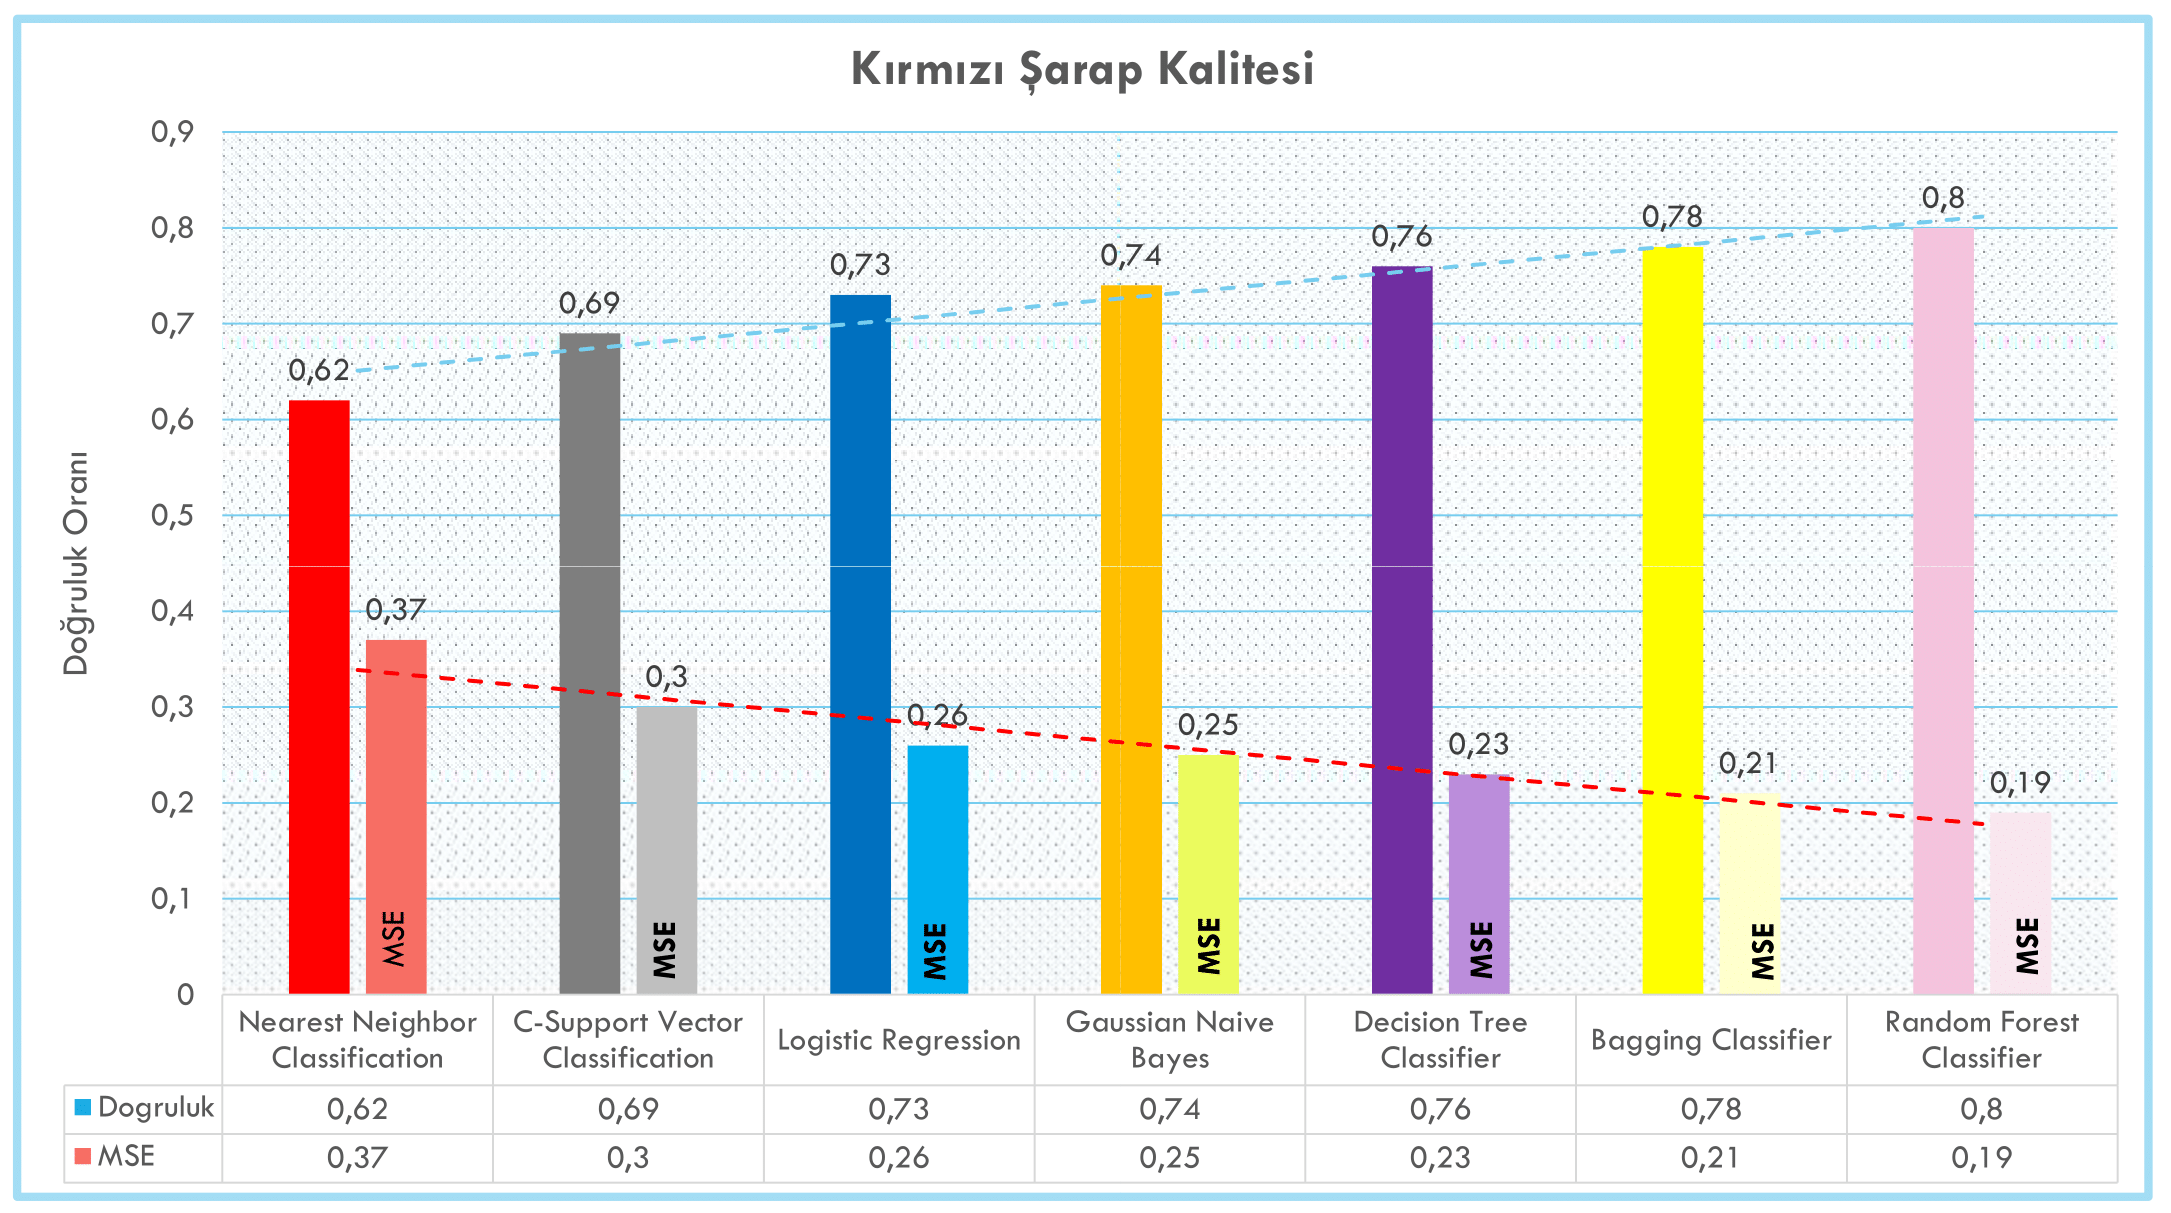
\includegraphics[scale=0.225]{pictures/pic_22.png}&
		\end{tabular}
	\end{center}
	\caption{Bagging Cross-Validation}
	\label{fig:22}
\end{figure}
\pagebreak
\begin{figure}[!h]
	\centering
	\begin{center}
		\begin{tabular}{cc}
			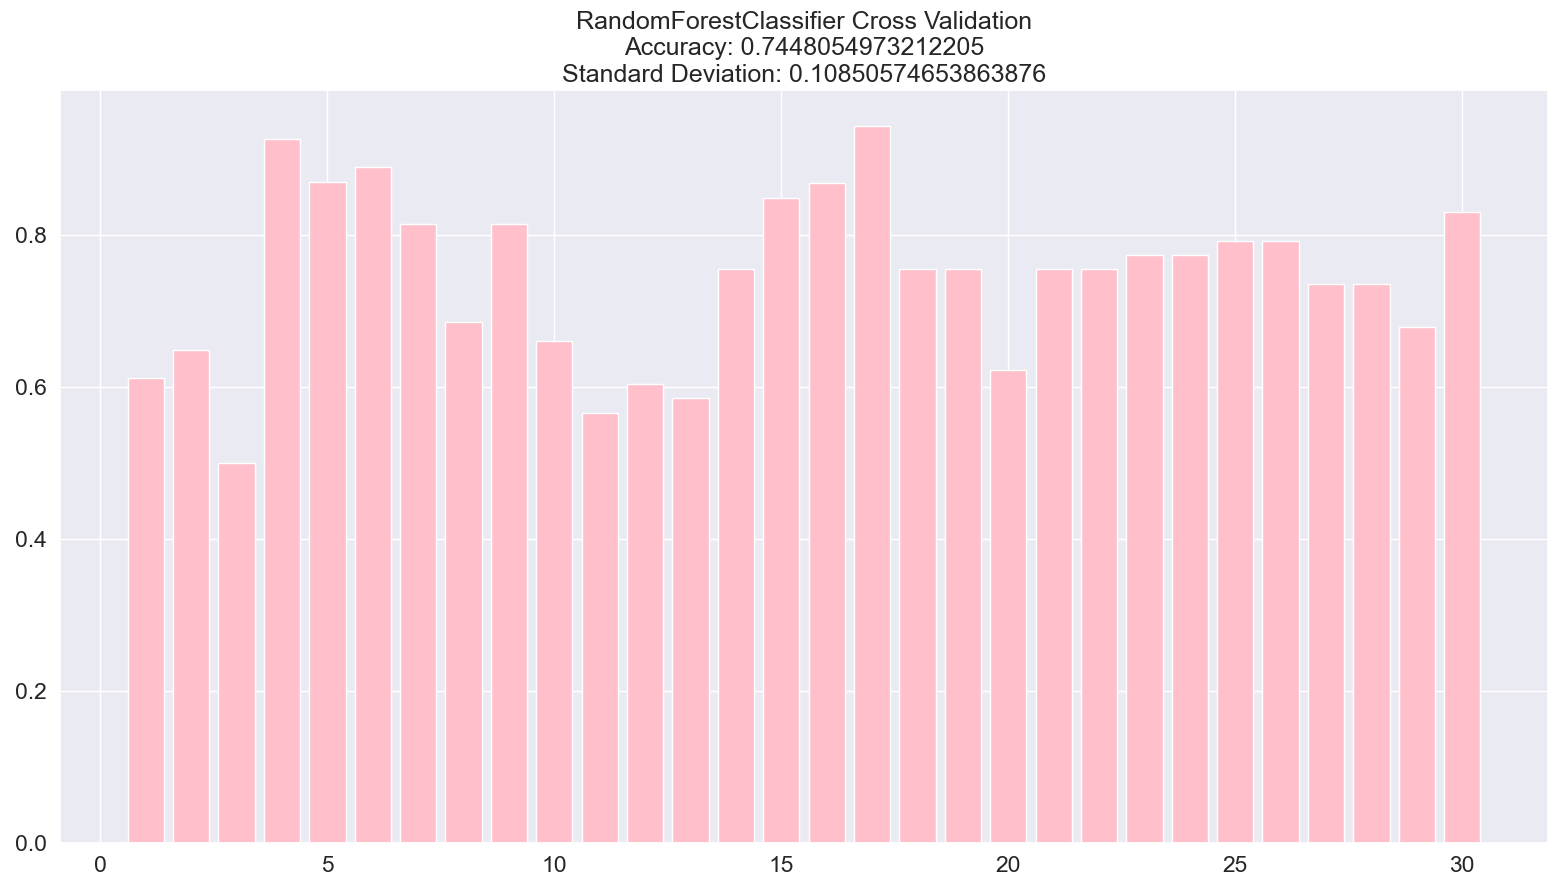
\includegraphics[scale=0.225]{pictures/pic_23.png}&
		\end{tabular}
	\end{center}
	\caption{Random Forest Tree Cross-Validation}
	\label{fig:23}
\end{figure}

\quad Bagg, DT, KNN, LG, NB, RF ve SVM algoritmaları \textbf{10 Kat Çapraz Doğrulama} yöntemi kullanarak eğitildi, çıkan sonuçlar ise Şekil \ref{fig:17}, \ref{fig:18}, \ref{fig:19}, \ref{fig:20}, \ref{fig:21}, \ref{fig:22} ve \ref{fig:23}'te görselleştirildi. Bu yöntem sonucunda;
\begin{itemize}
\item \textbf{Çalışma Sayısı}$(30) * $\textbf{Algoritma Sayısı}$(7) = \textbf{210}$
\end{itemize}
adet sonuç elde edildi. Bu sonuçların ortalama değerleri de Tablo \ref{tbl:02}'de belirtildi.

\begin{table}[h]
	\centering
	\normalsize
	\begin{tabular}{|l|c|c|c|c|}
		\hline
					& \textbf{acc}		& \textbf{St.Dev.}		\\ \hline
		\textbf{Bagg}	& 0.7004			& 0.0927			\\ \hline
		\textbf{DT}		& 0.6835			& \textbf{0.0840}		\\ \hline
		\textbf{KNN}	& 0.6928			& 0.0981 			\\ \hline
		\textbf{LG}		& 0.7336			& 0.0969			\\ \hline
		\textbf{NB}		& 0.7273			& 0.1139			\\ \hline
		\textbf{RF}		& \textbf{0.7448}		& 0.1090			\\ \hline
		\textbf{SVM}	& 0.7291			& 0.0957			\\ \hline
	\end{tabular}
	\caption{Bagging, DT, KNN, LG, NB, RF ve SVM sınıflandırıcılarının \textbf{Cross-Validation (10 Kat Çapraz Doğrulama)} sonuçlarının ortalama değerleri}
	\label{tbl:02}
\end{table}

\textbf{Standard Devination (Standart Sapma): } Değişken veri değerlerinin yayılımı özetlemek için kullanılır. Formülü Eşitlik\ref{eq:08}’teki gibidir.

\begin{equation}
\label{eq:08}
\Large \sigma= \sqrt{E((X-E(X))_{}^{2})}
\end{equation}

\quad Tablo \ref{tbl:02}'deki değerlere bakıldığı zaman en yüksek doğruluk ortalamasına sahip algoritmanın Random Forest $(0.7448)$ ve en düşük standart sapma ortalamasına sahip algoritmanın da Decision Tree $(0.0840)$ olduğu görülmektedir.

\quad Bagging algoritmasının $acc$ değerlerine bakıldığı zaman diğer algoritmaların ortalamasının üstünde kaldığını ve $StandardDevination$ değerinin de diğer algoritmaların ortalamasının altında kaldığı görülmektedir. Bu senaryoda en verimli algoritmalardan birinin de Bagging olduğu söylenebilir.


%%%%%%%%%%%%%%%%%%%%

\pagebreak

\section{\textbf{SONUÇ}}
\quad Bu projede kullanılan veri seti sayesinde kırmızı şarabın kalitesinin, ortalamanın üstünde veya altında olduğu tahmin edilmeye çalışılmıştır. Bunu yapmak için, önceden belirlenen algoritmalar kullanıldı ve sonuçları karşılaştırıldı. Her algoritmada farklı doğruluk değerleri elde edilmiştir. Bazı algoritmalar bu veri seti için daha yeterli olurken bazıları daha yetersiz kaldı. Algoritmaların veri setiyle verimli çalışabilmesi için, veri setinin detaylandırılması gerekir. Bunu da doğru özniteliklerin eklenmesi veya çıkartılması, örnek sayısının çoğaltılmasıyla sağlanabilir. Bu sayede kalite ölçümü daha efektif hale getirilebilir.

\begin{figure}[!h]
	\centering
	\begin{center}
		\begin{tabular}{cc}
			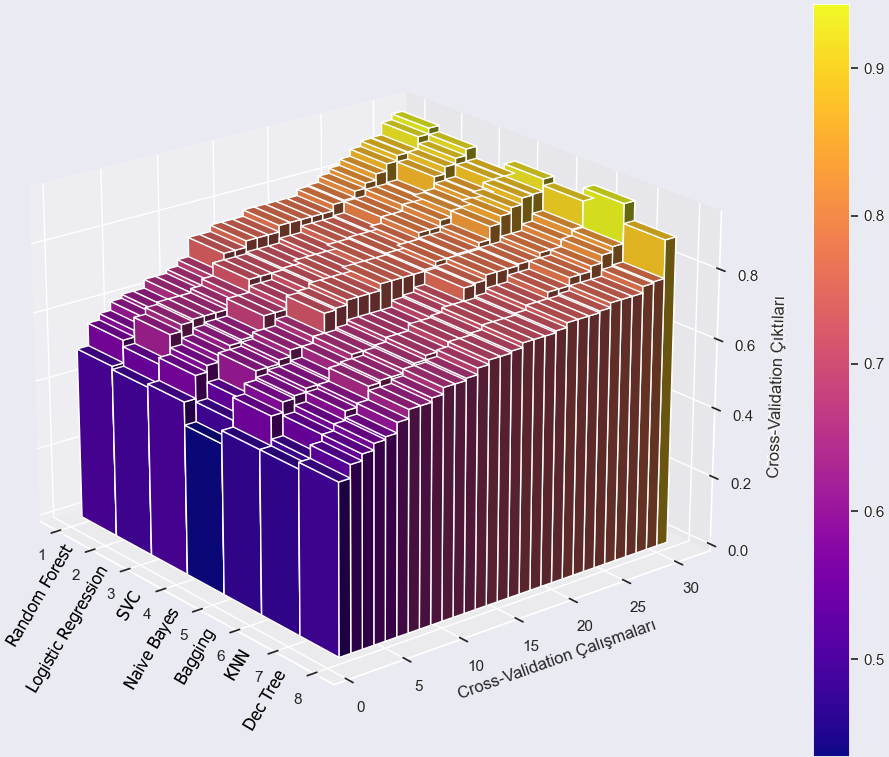
\includegraphics[scale=0.375]{pictures/pic_24.png}&
		\end{tabular}
	\end{center}
	\caption{Tüm Algoritmaların Cross-Validation Sonuçlarının 3D Grafiği}
	\label{fig:24}
\end{figure}

\quad $X-ekseni$'ne bakıldığı zaman algoritmaların isimleri, $Y-ekseni$'ne bakıldığında ise bu algoritmaların çalışma sayıları görülmektedir. Eldeki $X-Y$ şeklindeki 2D ortama 3. bir boyut$(Z-ekseni)$ olarak, bu algoritmaların çalışma sonuçları da eklendi.

\quad 3D grafik incelenirse, en yüksek ortalamaya sahip algoritmanın Random Forest olduğu anlaşılır. Çalışma sonuçları küçükten büyüğe sıralanarak bir rampa oluşması sağlandı. Bu sayede rampanın yüksek kısmında kalan algoritmalar, yüksek verimliliğe sahip algoritmalar oldu.

\begin{table}[h]
	\centering
		\normalsize
\begin{tabular}{|c|cc|cc|}
\hline


\multirow{2}{*}{}          & \multicolumn{2}{c|}{\textbf{Mevcut Proje}}      & \multicolumn{2}{c|}{\textbf{gollakeerthana}}         \\ \cline{2-5} 
                           & \multicolumn{1}{c|}{\textbf{acc}} & \textbf{St.Dev.} & \multicolumn{1}{c|}{\textbf{acc}} & \textbf{St.Dev.} \\ \hline
\textbf{Random Forest}     & \multicolumn{1}{c|}{\textbf{0.7448}}      & 0.1090       & \multicolumn{1}{c|}{\textbf{0.6875}}      & N/A       \\ \hline
\textbf{Logistic Regression} & \multicolumn{1}{c|}{0.7336}      & \textbf{0.0969}       & \multicolumn{1}{c|}{0.5854}      & N/A       \\ \hline
\end{tabular}
\caption{\textbf{gollakeerthana} kullanıcısının eğitim sonuçları\cite{23} ile karşılaştırma}
	\label{tbl:03}
\end{table}

\quad Ortak veri seti kullanılan bir kullanıcının eğitim sonuçları\cite{23} ile elde edilen sonuçlar karşılaştırılırsa, çok daha iyi bir sonuç elde edildiği görülebilir. Bunun sebebi veri seti üzerinde gerçekleştirilen önişleme adımlarıdır.

%%%%%%%%%%%%%%%%%%%%

\newpage
\begin{thebibliography}{23}

\bibitem{1} 
DergiPark - Şarap Üretimi ve Kalite
\\\texttt{\href{https://dergipark.org.tr/tr/download/article-file/498270}{\nolinkurl{dergipark.org.tr/sarap-uretimi-ve-kalite}}}

\bibitem{2} 
Wikipedia - Şarap
\\\texttt{\href{https://tr.wikipedia.org/wiki/Şarap}{\nolinkurl{wikipedia.org/Şarap}}}

\bibitem{3} 
Resmi Gazete - Türk Gıda Kodeksi Şarap Tebliği
\\\texttt{\href{https://www.resmigazete.gov.tr/eskiler/2009/02/20090204-12.htm}{\nolinkurl{resmigazete.gov.tr/2009/02/20090204-12}}}

\bibitem{4} 
Kaggle - Red Wine Quality Dataset
\\\texttt{\href{https://www.kaggle.com/uciml/red-wine-quality-cortez-et-al-2009}{\nolinkurl{kaggle.com/red-wine-quality}}}

\bibitem{5} 
Wine Quality Exploration
\\\texttt{\href{http://rstudio-pubs-static.s3.amazonaws.com/80458_5000e31f84df449099a872ccf40747b7.html}{\nolinkurl{amazonaws.com/wine-quality-exploration}}}

\bibitem{6} 
Hydrometer Confusion
\\\texttt{\href{http://www.creativeconnoisseur.com/newsletter/files/497deafe6be1b2efc87df8ac6071e459-162.html}{\nolinkurl{creativeconnoisseur.com/hydrometer-confusion}}}

\bibitem{7} 
Erdal Taşçı \& Aytuğ Onan - KNN Algorithm
\\\texttt{\href{https://ab.org.tr/ab16/bildiri/102.pdf}{\nolinkurl{ab.org.tr/knn-algorithm}}}

\bibitem{8} 
Scholarpedia - K-Nearest Neighbor
\\\texttt{\href{http://scholarpedia.org/article/K-nearest_neighbor}{\nolinkurl{scholarpedia.org/K-nearest_neighbor}}}

\bibitem{9} 
Erdinç Uzun - KNN Algoritması
\\\texttt{\href{https://erdincuzun.com/makine_ogrenmesi/k-nn-algoritmasi/}{\nolinkurl{erdincuzun.com/makine_ogrenmesi/k-nn-algoritmasi}}}

\bibitem{10} 
Large Margin Nearest Neighbor Classification
\\\texttt{\href{https://proceedings.neurips.cc/paper/2005/file/a7f592cef8b130a6967a90617db5681b-Paper.pdf}{\nolinkurl{proceedings.neurips.cc/Margin_Nearest_Neighbor_Classification.pdf}}}

\bibitem{11} 
DergiPark - Destek Vektör Makinesi
\\\texttt{\href{https://dergipark.org.tr/tr/download/article-file/65371}{\nolinkurl{dergipark.org.tr/Destek_Vektor_Makinesi}}}

\bibitem{12} 
Medium - Destek Vektör Makineleri
\\\texttt{\href{https://medium.com/deep-learning-turkiye/nedir-bu-destek-vektör-makineleri-makine-öğrenmesi-serisi-2-94e576e4223e}{\nolinkurl{medium.com/deep-learning-turkiye/destek-vektör-makineleri}}}

\bibitem{13} 
Medium - Lojistik Regresyon
\\\texttt{\href{https://medium.com/@k.ulgen90/lojistik-regresyon-makine-öğrenimi-bölüm-7-c6bc685a4084}{\nolinkurl{medium.com/lojistik-regresyon-makine-öğrenimi}}}

\bibitem{14} 
Başken Üniversitesi - Naive Bayes
\\\texttt{\href{https://mail.baskent.edu.tr/~20410964/DM_9.pdf}{\nolinkurl{baskent.edu.tr/Naive_Bayes.pdf}}}

\bibitem{15} 
Akademik Bilişim - Naive Bayes
\\\texttt{\href{https://ab.org.tr/ab14/bildiri/186.pdf}{\nolinkurl{ab.org.tr/Naive_Bayes.pdf}}}

\bibitem{16} 
Medium - Karar Ağaçları
\\\texttt{\href{https://medium.com/@k.ulgen90/makine-öğrenimi-bölüm-5-karar-ağaçları-c90bd7593010}{\nolinkurl{medium.com/makine-öğrenimi-karar-ağaçları}}}

\bibitem{17} 
Sosyal Araştırmalar - Karar Ağacı
\\\texttt{\href{https://www.sosyalarastirmalar.com/articles/text-classification-via-decision-trees-algorithm-customer-comments-case.pdf}{\nolinkurl{sosyalarastirmalar.com/decision-trees-algorithm}}}

\bibitem{18} 
Medium - Ensemble Learning
\\\texttt{\href{https://medium.com/deep-learning-turkiye/ensemble-learning-bagging-ve-boosting-50643428b22b}{\nolinkurl{medium.com/ensemble-learning-bagging-ve-boosting}}}

\bibitem{19} 
Medium - Rastgele Orman Ağacı Algoritması
\\\texttt{\href{https://medium.com/@cemthecebi/rastgele-orman-algoritması-1600ca4f4784}{\nolinkurl{medium.com/rastgele-orman-algoritması}}}

\bibitem{20} 
DevHunter - Rastgele Orman Ağacı Algoritması
\\\texttt{\href{https://devhunteryz.wordpress.com/2018/09/20/rastgele-ormanrandom-forest-algoritmasi/comment-page-1}{\nolinkurl{devhunteryz.com/rastgele-ormanrandom-forest-algoritmasi}}}

\bibitem{21} 
SlideShare - Rastgele Orman Ağacı Algoritması
\\\texttt{\href{https://www.slideshare.net/SezerFidanc/random-forest-algoritmas}{\nolinkurl{slideshare.net/random-forest-algoritması}}}

\bibitem{22} 
Medium - ROC Eğrisi
\\\texttt{\href{https://bernatas.medium.com/roc-eğrisi-ve-eğri-altında-kalan-alan-auc-97b058e8e0cf}{\nolinkurl{medium.com/roc-eğrisi}}}

\bibitem{23} 
Kaggle - Red Wine Quality
\\\texttt{\href{https://www.kaggle.com/gollakeerthana/red-wine-quality-lr-rf-93}{\nolinkurl{kaggle.com/gollakeerthana/red-wine-quality}}}



\end{thebibliography}

\end{document}
